% !TEX TS-program = pdflatex
% !TEX encoding = UTF-8 Unicode

% This is a simple template for a LaTeX document using the "article" class.
% See "book", "report", "letter" for other types of document.

% use larger type; default would be 10pt
\documentclass[11pt]{scrartcl}

% set input encoding (not needed with XeLaTeX)
\usepackage[utf8]{inputenc}
\usepackage[title,titletoc,header]{appendix}
\usepackage{multicol}
% \usepackage{titling}
\usepackage{longtable}

\usepackage{amsmath}
\usepackage{hyperref}

\usepackage{todonotes}
\presetkeys{todonotes}{inline}{}

\usepackage{natbib}
% To cite, use \citet{} in text citation, or \citep{} (in parentheses).

%%% PAGE DIMENSIONS
\usepackage[a4paper]{geometry} % to change the page dimensions
% \geometry{a4paper, margin=1.3in} % or letterpaper (US) or a5paper or....
% \geometry{margin=2in} % for example, change the margins to 2 inches all round
% \geometry{landscape} % set up the page for landscape
%   read geometry.pdf for detailed page layout information

\usepackage{graphicx} 				% support the \includegraphics command and options

% \usepackage[parfill]{parskip} % Activate to begin paragraphs with an empty line rather than an indent

%%% PACKAGES
\usepackage{booktabs} 				% for much better looking tables
\usepackage{array} 					% for better arrays (eg matrices) in maths
\usepackage{paralist} 				% very flexible & customisable lists (eg. enumerate/itemize, etc.)
\usepackage{verbatim} 				% adds environment for commenting out blocks of text & for better verbatim
\usepackage{subfig} 				% make it possible to include more than one captioned figure/table in a single float
\usepackage{float} 					% allow floating for figures

\usepackage{pgfgantt} 				% gantt charts
% \usepackage[export]{adjustbox}[2011/08/13] % For centering wide figures

%%% PARAGRAPHING & INDENTATION
\setlength{\parindent}{0pt}
\setlength{\parskip}{2ex plus 0.5ex minus 0.3ex}

%%% HEADERS & FOOTERS
\usepackage{fancyhdr} 				% This should be set AFTER setting up the page geometry
\pagestyle{fancy} 					% options: empty , plain , fancy
\renewcommand{\headrulewidth}{0pt} 	% customise the layout...
\lhead{}\chead{}\rhead{}
\lfoot{}\cfoot{\thepage}\rfoot{}

%%% SECTION TITLE APPEARANCE
\usepackage{sectsty}
\allsectionsfont{\sffamily\mdseries\upshape} % (See the fntguide.pdf for font help)
% (This matches ConTeXt defaults)

%%% ABSTRACT APPEARANCE
\usepackage{abstract}
\renewcommand{\absnamepos}{flushleft}
\setlength{\absleftindent}{0pt}
\setlength{\absrightindent}{0pt}

%%% TABLE OF CONTENTS APPEARANCE
 % Put the bibliography in the ToC
\usepackage[nottoc,notlof,notlot]{tocbibind}
 % Alter the style of the Table of Contents
\usepackage[titles,subfigure]{tocloft}
\renewcommand{\cftsecfont}{\rmfamily\mdseries\upshape}
 % No bold!
\renewcommand{\cftsecpagefont}{\rmfamily\mdseries\upshape}

%%% REFERENCES APPEARANCE
\renewcommand{\bibname}{References}

\newcommand{\code}[1]{{\texttt{#1}}}
\newcommand{\libraryname}[1]{{\texttt{#1}}}
\newcommand{\codefile}[1]{{\textit{#1}}}
\newcommand{\program}[1]{\code{#1}}
\newcommand{\taskname}[1]{{\textit{#1}}}

\title{Shading-Based Sphere Detection}
\subtitle{Computer Vision Project Proposal}
\author{Brendan Annable, Mitchell Metcalfe, Monica Olejniczak}

% Activate to display a given date or no date (if empty), otherwise the current date is printed
\date{\today}

\rhead{COMP4110, Project Proposal, \today}

\begin{document}
	\maketitle

	\begin{abstract}
		This proposal researches current methods of sphere detection and proposes 
		the use of boosted weak classifiers based on these findings. This report 
		describes this method and how its development will be approached. The
		dataset will be created in-house and must include a broad 
		range of image features, environments and lighting conditions to ensure
		that the results can be well tested. The timeline of this proposal is
		detailed, as well as the roles and responsibilities of the researchers
		and how the results will be communicated.
	\end{abstract}

	\newpage
	\tableofcontents
	\newpage

	\section{Summary} {
        
        This project aims to develop software that is capable of detecting spheres within a given image. Instead of the more common approach of using the sphere's colour, this project will investigate the idea of using the shading of the sphere for detection. Removing the dependency on colour should improve robustness and reduce false positives.
        
        A robust sphere detection algorithm would be of interest in many robotics applications, for example the RoboCup international robot soccer competition, where the robots must be able to track a soccer ball in real-time in order to compete. It would also be of interest to human players in competitive sports environments, such as basketball or tennis, where automatic cameras are used to accurately make referee calls based on whether a ball had gone out or not.
        
        If the methods developed are efficient and perform well enough, they can be expected to be implemented by the Newcastle Robotics Laboratory's RoboCup team, the NUbots.
		
	}

	\section{Background and aims} {

  		Visually keeping track of a ball is a natural and fundamental aspect of playing 
  		soccer, that many human players would not consider to be a skill in itself. 
  		However, while it may come naturally to humans, fast and reliable ball
        tracking has presented a challenge that has attracted much research in
        the robot soccer community.
        
        % % Note: This is largely achieved by the remainder of this section.
        % \todo { 
        %     Refer to the progression of ball detection techniques from colour based to
        %     shape based and intensity based.

        %     Describe our approach as a natural
        %     next step.
        % }

        Early attempts at ball detection algorithms used in the international robot soccer competition,
        RoboCup, simply used histogramming techniques targeted at a specific range of colour intensities to find a coloured ball. As the RoboCup playing field has become less structured over the years, competing teams have needed to account for unpredictable colours and have increasingly implemented methods that detect the shape of the ball as well.
        \citet{schulz2007ball} used a neural network on
        subsampled luminance images of the ball to detect the shape of the 
        ball. Recent approaches have focused on detecting the approximately
        circular shape of the ball in typical images. These include
        clustering, hough filters \citet{li2013survey}, and RANSAC.

        \todo {
            Make a note about colour classification: 

            "The preprocessing step of colour classification using a precalculated
            lookup table has become standard in the Standard Platform and Kid Size
            leagues."
        }

        Many current ball detection methods make assumptions about the ball or
        the environment that limit their applicability in a more general case. Methods
        based on colour classification or similarity can suffer from false
        positive detections due to other objects having similar colours. These methods may 
        also detect both false positives and false negatives due to unexpected changes
        in lighting. Methods based on circle or ellipse detection can be effected by
        false positives due to the presence of disk-like objects in the
        environment, or due to objects that appear circular when viewed from
        specific angles.

        % % Note: These comments are probably unnecessary.
        % \todo {
        %     Posit the circular appearance of disk-like objects as the worst
        %     case for current ball-detection methods.
        % }
        % \todo { 
        %     Hypothesise that spatial relationships between separate 3D features (e.g.
        %     specular highlight, shadow, shading gradient, the projected ellipse)
        %     should help to identify spheres, as they have helped in detecting faces.
        % }

        To avoid the limitations of methods based on assumptions such as
        these, we propose to research and develop a sphere detection method which uses
        the shading patterns characteristic of spherical objects to classify
        objects as spheres.

        \citet{nillius2008shading} perform shading based sphere detection
        using Principal Component Analysis (PCA) with a basis derived analytically from a given Bidirectional Reflectance Distribution Function (BRDF) and assumptions
        on scene illumination. While this method works well for plain untextured spheres, it is
        not designed to work on spheres with patterns printed on them, like many
        soccer balls.

        To build a detector that is more robust to differently textured
        spheres, we plan to investigate the application of techniques
        popularised in the realm of face detection to the task of sphere
        detection. We consider this a promising approach, because the 3D
        features of spheres tend to have similar spatial constraints to facial
        features in many cases.

        For simplicity, the scope of the proposed project is limited to the
        common and important case of detecting balls that are resting on the
        ground. We will also assume that the sphere is illuminated primarily
        from above to constrain the likely positions of shadows and specular
        highlights.

        \citet{masselli2013haar} successfully apply a boosted Haar classifier
        \citep{viola2001robust} to the problem of ball recognition. They show
        that the Haar classifier outperformed a more classical approach, based on a
        Hough transform, in the task of detecting uniformly yellow, green, and white
        balls.

        \citet{zhang2013novel} used a similar approach, but attempted to
        detect a wide variety of generic FIFA-style balls. They used extended
        Haar features \citep{Lienhart2002extended} as weak classifiers.
        \citeauthor{zhang2013novel} reported improved performance when modified Haar
        features that used a division operation between their area sums, instead of
        the usual subtraction, were included. This suggests that exploring alternate
        weak classifiers could lead to valuable performance improvements.

        \citet{mitri2004fast} applied a Sobel filter and a threshold function
        to each image as preprocessing steps, passing only the detected edge
        images to the classifiers. The method learnt Classification and
        Regression Trees (CARTs) of Haar features instead of directly using
        Haar features as weak classifiers. Their system performed sufficiently
        well for ball tracking, but detected other round objects as false
        positives. It also performed significantly better when a more complex
        training dataset was applied, which included images under different 
        lighting conditions and environments. We consider it likely that their 
        poor false positive rate was a symptom of ignoring the shading 
        information of the spheres by using only an edge image.

        \citet{Treptow2004filter} achieved a much lower false positive rate
        using Haar features directly, but only trained and tested their
        detector on a single ball.

        % % Note: Let's not do this. It's a bit too strong/unlikely to work.
        % %       We should instead just mention patch descriptors as a possible
        % %       technique in the project plan?
        % \todo {
        %     Hypothesise that local feature/patch descriptors should be enough
        %     to identify the specular highlight and shadow cast by a sphere.
        % }

        \todo {
            Contrast the goal of our proposed project with the focus of most other
            algorithms, which generally do not attempt to verify that they have not
            erroneously detected disks.

            The below sentence may be enough?
        }

        As a result of targeting our approach toward the 3D features that
        distinguish spheres from objects such as disks, we expect our method
        to be particularly robust against detecting false positives.
	}

	\section{Project plan} {
    \label{sec:plan}

        % % Note: Not sure about this anymore. As our project is now focused
        % % on differentiating spheres and disks, rather than execution time,
        % % adding this to the proposal seems like adding unnecessary work. We
        % % could talk about these in the next report if they become
        % % important/things are going well/our topic changes?
        % \todo {
        %     Outline the tendency of ball and face detection approaches to use a
        %     coarse/cheap candidate detection pass and a more accurate/costly
        %     verification/outlier rejection pass, and propose that we follow the
        %     same approach and investigate one or two alternatives (Hough
        %     transform, \citet{Yuan2015} or \citet{Pan2011}, a more ad-hoc
        %     method?) and compare results - possibly by leveraging the NUbots'
        %     existing system.
        % }

        % exploring the relative effectiveness of different weak classifiers
        % and patch descriptors in training boosted classifiers to
        % differentiate spheres and other round objects

        We plan to develop a sphere detection system based on boosted weak
        classifiers in the style of \citeauthor{zhang2013novel}, and
        \citeauthor{masselli2013haar}, but with the additional goal of
        distinguishing spheres from objects of similar appearance such as
        disks. Due to the increased difficulty of this classification task, we
        plan to investigate a variety of weak classifiers for use in the
        adaboost algorithm. Successful classifier options we plan to explore
        include the extended Haar features used by \citet{zhang2013novel},
        Histograms of Oriented Gradients (HoG) features, as used in
        \citet{zhu2006hogs}, and variations on more recent patch descriptors such
        as the ORB descriptor introduced by \citet{rublee2011orb}.


        \todo {
            Outline how the methods proposed will be evaluated and compared, with
            reference to any expected difficulties.
        }

        We will train and test our sphere detector on a purpose built image database.

        \subsection{Image dataset creation} {

        	The creation of the dataset will be built by the research team, removing
        	the need for purchasing which eliminates any copyright and production
        	issues that could otherwise occur. This also enables the team to
        	create a consistent dataset.

        	The images will be taken using a Cannon EOS60D camera with varying
        	lighting conditions and environments to ensure a diverse dataset is
        	obtained. These photographs will be compressed using a high quality
        	format so that they are easier to process than the original without
        	losing much, if any, information.

        	Some images will be duplicated and altered using photo editing software,
        	for the sole purpose of testing the same image under various 
        	conditions. These modifications may change the quality of the image or
        	its lighting environment. A transformation to the image such as rotation
        	or scaling may also be applied.

            The dataset will include a number of images that contain a variety
            of spheres and disks. There will be a balance of object sizes,
            patterns, colours and textures between the images and can include
            the use of a tennis, soccer, golf and cricket ball. To reduce the
            complexity of this project, the images will be taken of motionless spheres, to avoid any motion blur.
            
            There is also the possibility of generating spheres procedurally, combing computer graphics and Physically Based Rendering \citep{pbr}, seen in Figure \ref{figure:pba}. This will provide an opportunity to thoroughly test and compare the detection methods on spheres with easily measurable and known characteristics. This method will be a low priority and used for the validation of results near the end of the project if time permits.
            
			\begin{figure}[H]            
				\centering
    	        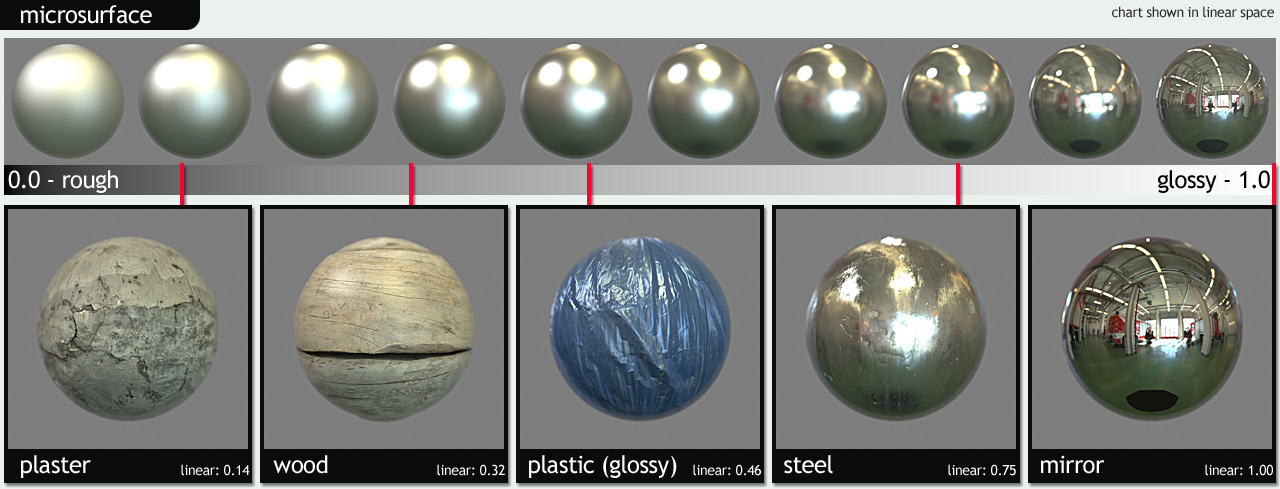
\includegraphics[width=13cm]{microcompare05.jpg}
	            \caption[Project Schedule] {
                	Generated spheres using Physically Based Rendering \citep{pbr}.
				}
				\label{figure:pba}
            \end{figure}
            
            Images of balls that are primarily metallic or
            transparent will also not be included in the initial dataset. To begin with, the images
            should contain an individual ball or disk and then progress to
            having both, or a combination of, within the same image. This will
            test whether our methods of detection are able to identify
            multiple spheres correctly. Some images may feature:

        	\begin{itemize}
        		\item Objects that appear as spheres from different angles.
        		\item Non-spherical objects.
        		\item An aspheric (deflated) sphere.
        		\item Spheres that intersect with each other.
        		\item Disks that intersect with each other.
        		\item A sphere and disk that intersect with each other.
        		\item A sphere or disk that is rotated.
        		\item A sphere or disk that is partially cropped out.
        	\end{itemize}

        	It is of significant importance to create a dataset that features an
        	array of environments, to ensure that the sphere detection methods are
        	robust and able to function in as many scenarios as possible. These
        	environments have been grouped into four distinct categories:

        	\begin{enumerate}
        		\item \textbf{Soccer:} This is a standard indoor robot soccer 
        		environment.
        		\item \textbf{Uniform:} The environment is plain and largely the same
        		colour.
        		\item \textbf{Textured:} The environment contains textures and
        		repeatable patterns.
        		\item \textbf{Cluttered:} The environment contains many objects that
        		may obscure the detection of spheres.
        	\end{enumerate}
        	
        	And may exhibit the following range of lighting conditions:

        	\begin{itemize}
        		\item The number of lights vary.
        		\item The position of the lights vary.
        		\item The scene is lit from a single light source.
        		\item The scene is lit from multiple light sources in a similar direction.
        		\item The scene is lit from multiple light sources from different directions.
        		\item The lighting is under normal conditions.
        		\item The lighting is dim.
        		\begin{itemize}
        			\item The shadow of the ball should blend with the environment.
        		\end{itemize}
        		\item The lighting is bright.
        		\begin{itemize}
        			\item The lighting of the ball should blend with the environment.
        		\end{itemize}
        	\end{itemize}

        	The dataset should also include a good combination of features and
        	environment configurations to test more complex cases. For example, two
        	intersecting spheres of the same colour under dim lighting will be far 
        	more difficult to identify than two individual spheres of differing
        	colours in good lighting. The texture of the sphere should also be
        	considered as it can effect the type of lighting that is emitted.

        	The positions and sizes of the spheres within the dataset will be
        	specified by drawing boxes around them, so these cropped images can be
        	used to train the classifiers.

        }

	}

	\section{Project schedule} {
        The project plan outlined in section~\ref{sec:plan} is to be achieved
        according to the schedule presented in the Gantt chart in
        Figure~\ref{gantt:proposal}.

        The project has 3 main phases:
        
        \begin{itemize}
        	\item Project proposal (2 weeks)
        	\item Project work (5 weeks)
        	\item Final report (4 weeks)
        \end{itemize}

		\begin{figure}[H]
	        \makebox[\textwidth][c]{\resizebox{0.95\paperwidth}{!}{% Define some Gantt chart helper commands:
\newcommand{\completedganttbar}[4][]{ %
    \ganttbar[bar/.append style={draw=gray, fill=gray},#1]{#2}{#3}{#4} %
}
\newcommand{\optionalganttbar}[4][]{ %
    \ganttbar[bar/.append style={draw=gray, pattern color=gray, pattern=north west lines},#1]{#2}{#3}{#4} %
}
\newcommand{\optionalganttlinkedbar}[4][]{ %
    \ganttlinkedbar[bar/.append style={draw=gray, pattern color=gray, pattern=north west lines},#1]{#2}{#3}{#4} %
}

\begin{ganttchart}[
        hgrid,
        vgrid={*6{black, dotted},*1{black, dashed}}, % Note: NO SPACES!
        title height = 1,
        x unit=0.3cm,
        y unit title=0.75cm,
        y unit chart=1cm,
        time slot format=isodate,
        % progress=today,
        % today=2015-8-20,
        % bar/.append style={fill=green},
        % bar incomplete/.append style={fill=white},
        % group incomplete/.append style={draw=black,fill=none},
        % progress label text={}
        ]
        {2015-03-16} % start date: Mon, Mar-16. Week 4.
        {2015-05-31} % end date: Sun, May-31.
\setganttlinklabel{f-s}{}

% Gantt chart header:
% Note: Week starts on Sunday.
\gantttitlecalendar*{2015-03-16}{2015-05-31}{month=name} \\
\gantttitlecalendar*{2015-03-16}{2015-04-05}{week=4}
\gantttitle{Semester 1 Recess}{14}
\gantttitlecalendar*{2015-04-20}{2015-05-31}{week=7}

% Proposal
\ganttnewline \ganttgroup{Project proposal}{2015-03-19}{2015-03-26}
\ganttnewline \ganttbar{Report}{2015-03-19}{2015-03-23}
\ganttnewline \ganttbar{Presentation}{2015-03-24}{2015-03-26}

% Project work
\ganttnewline \ganttgroup{Project work}{2015-03-27}{2015-04-30}
\ganttnewline \ganttbar{Dataset collection}{2015-03-27}{2015-04-05}
\ganttnewline \ganttbar{Candidate selection}{2015-04-01}{2015-04-08}
\ganttnewline \ganttbar{Development}{2015-04-09}{2015-04-22}
\ganttnewline \ganttbar{Report preparation}{2015-04-23}{2015-04-30}

% Final report
\ganttnewline \ganttgroup{Final report}{2015-04-31}{2015-05-28}
\ganttnewline \ganttbar{Detection performance testing}{2015-04-31}{2015-05-07}
\ganttnewline \ganttbar{Analysis of results}{2015-05-08}{2015-05-15}
\ganttnewline \ganttbar{Report preparation}{2015-05-16}{2015-05-28}

% % Examples of gantt chart capabilities: 
% \ganttnewline \ganttgroup{Label Text}{2015-08-20}{2015-10-5}
% \ganttnewline \ganttmilestone{Label Text}{2015-08-3}
% \ganttnewline \completedganttbar{Label Text}{2015-8-9}{2015-8-13}
% \ganttnewline \ganttlinkedmilestone{Label Text}{2015-08-19}
% \ganttnewline \ganttbar{Label Text}{2015-09-11}{2015-10-5}
% \ganttnewline \optionalganttbar{Label Text}{2015-10-6}{2015-10-26}

\end{ganttchart}
}}
			\caption[Project Schedule] {
                A Gantt chart illustrating the planned project schedule.
			}
			\label{gantt:proposal}
		\end{figure}
	}

	\section{Roles and responsibilities} {

		Given the small size of the team, it will be easier to distribute the workload evenly if no particularly role is assigned to an individual. This means each researcher will equally contribute to the research, development and documentation of the project. Each researcher is committed to spending on average 8 hours of work per week to ensure that the project is completed on schedule.
		
		Researchers will seek academic advice from their supervisors and colleagues if and when necessary.
    }

    \section{Communication of results} {

        The results of the project will be compiled into a report, as outlined
        in the project schedule, that is intended to be suitable for
        submission to a relevant conference or journal. In the case that the
        report is accepted for publication, the dataset created for the
        project will also be made available online, along with the associated code.
        
    }

	\bibliography{bibliography}
	\bibliographystyle{apalike}

\end{document}

